\chapter{循环神经网络}\label{chap:Recu}

\begin{introduction}
	\item 递归神经网络是啥~\ref{Recu:1}
	\item 递归神经网络的前向计算~\ref{Recu:2}
	\item 递归神经网络的训练~\ref{Recu:3}
	\item 误差项的传递~\ref{Recu:4}
	\item 权重梯度的计算~\ref{Recu:5}
	\item 权重更新~\ref{Recu:6}
	\item 编程实战:递归神经网络的实现~\ref{Recu:7}
	\item 递归神经网络的应用~\ref{Recu:8}
	\item 自然语言和自然场景解析~\ref{Recu:9}
\end{introduction}




在前面的文章中,我们介绍了\textbf{循环神经网络},它可以用来处理包含序列结构的信息。然而,除此之外,信息往往还存在着诸如树结构、图结构等更复杂的结构。对于这种复杂的结构,\textbf{循环神经网络}就无能为力了。本文介绍一种更为强大、复杂的神经网络:\textbf{递归神经网络 (Recursive Neural Network, RNN)},以及它的训练算法\textbf{BPTS (Back
	Propagation Through Structure)}。顾名思义,\textbf{递归神经网络}(巧合的是,它的缩写和\textbf{循环神经网络}一样,也是RNN)可以处理诸如树、图这样的\textbf{递归结构}。在文章的最后,我们将实现一个\textbf{递归神经网络},并介绍它的几个应用场景。

\section{递归神经网络是啥}\label{Recu:1}

因为神经网络的输入层单元个数是固定的,因此必须用循环或者递归的方式来处理长度可变的输入。\textbf{循环神经网络}实现了前者,通过将长度不定的输入分割为等长度的小块,然后再依次的输入到网络中,从而实现了神经网络对变长输入的处理。一个典型的例子是,当我们处理一句话的时候,我们可以把一句话看作是词组成的序列,然后,每次向\textbf{循环神经网络}输入一个词,如此循环直至整句话输入完毕,\textbf{循环神经网络}将产生对应的输出。如此,我们就能处理任意长度的句子了。如图\ref{fig:Recu1}所示:

\begin{figure}[!h]
	\centering
	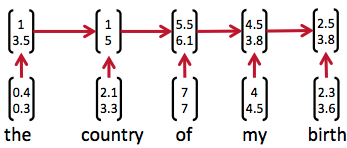
\includegraphics[width=0.7\textwidth]{Recu1.png}
	\caption{句子处理过程}
	\label{fig:Recu1}
\end{figure}

然而,有时候把句子看做是词的序列是不够的,比如下面图\ref{fig:Recu2}这句话『两个外语学院的学生』:

\begin{figure}[!h]
	\centering
	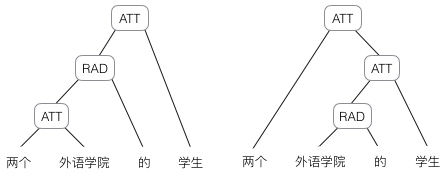
\includegraphics[width=0.7\textwidth]{Recu2.png}
	\caption{两个外语学院的学生}
	\label{fig:Recu2}
\end{figure}

图\ref{fig:Recu1}显示了这句话的两个不同的语法解析树。可以看出来这句话有歧义,不同的语法解析树则对应了不同的意思。一个是『两个外语学院的/学生』,也就是学生可能有许多,但他们来自于两所外语学校;另一个是『两个/外语学院的学生』,也就是只有两个学生,他们是外语学院的。为了能够让模型区分出两个不同的意思,我们的模型必须能够按照树结构去处理信息,而不是序列,这就是\textbf{递归神经网络}的作用。当面对按照树/图结构处理信息更有效的任务时,\textbf{递归神经网络}通常都会获得不错的结果。

\textbf{递归神经网络}可以把一个树/图结构信息编码为一个向量,也就是把信息映射到一个语义向量空间中。这个语义向量空间满足某类性质,比如语义相似的向量距离更近。也就是说,如果两句话(尽管内容不同)它的意思是相似的,那么把它们分别编码后的两个向量的距离也相近;反之,如果两句话的意思截然不同,那么编码后向量的距离则很远。如图\ref{fig:Recu3}所示:

\begin{figure}[!h]
	\centering
	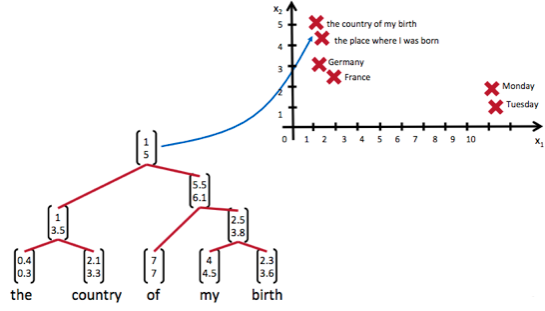
\includegraphics[width=0.7\textwidth]{Recu3.png}
	\caption{编码后向量的距离}
	\label{fig:Recu3}
\end{figure}

从图\ref{fig:Recu3}我们可以看到,\textbf{递归神经网络}将所有的词、句都映射到一个2维向量空间中。句子『the country of my birth』和句子『the place where I was born』的意思是非常接近的,所以表示它们的两个向量在向量空间中的距离很近。另外两个词『Germany』和『France』因为表示的都是地点,它们的向量与上面两句话的向量的距离,就比另外两个表示时间的词『Monday』和『Tuesday』的向量的距离近得多。这样,通过向量的距离,就得到了一种语义的表示。

上图还显示了自然语言\textbf{可组合}的性质:词可以组成句、句可以组成段落、段落可以组成篇章,而更高层的语义取决于底层的语义以及它们的组合方式。\textbf{递归神经网络}是一种表示学习,它可以将词、句、段、篇按照他们的语义映射到同一个向量空间中,也就是把可组合(树/图结构)的信息表示为一个个有意义的向量。比如上面这个例子,\textbf{递归神经网络}把句子"the
country of my birth"表示为二维向量{[}1,5{]}。有了这个『编码器』之后,我们就可以以这些有意义的向量为基础去完成更高级的任务(比如情感分析等)。如下图所示,\textbf{递归神经网络}在做情感分析时,可以比较好的处理否定句,这是胜过其他一些模型的:

\begin{figure}[!h]
	\centering
	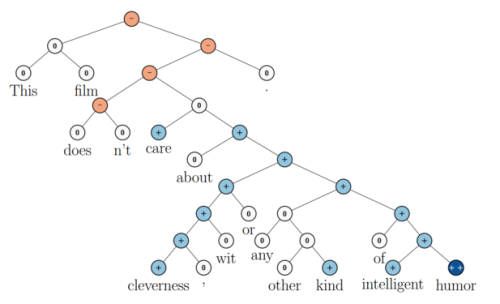
\includegraphics[width=0.7\textwidth]{Recu4.png}
	\caption{递归神经网络}
	\label{fig:Recu4}
\end{figure}

在图\ref{fig:Recu4}中,蓝色表示正面评价,红色表示负面评价。每个节点是一个向量,这个向量表达了以它为根的子树的情感评价。比如"intelligent humor"是正面评价,而"care about cleverness wit or any other kind of intelligent humor"是中性评价。我们可以看到,模型能够正确的处理doesn\'t的含义,将正面评价转变为负面评价。

尽管\textbf{递归神经网络}具有更为强大的表示能力,但是在实际应用中并不太流行。其中一个主要原因是,\textbf{递归神经网络}的输入是树/图结构,而这种结构需要花费很多人工去标注。想象一下,如果我们用\textbf{循环神经网络}处理句子,那么我们可以直接把句子作为输入。然而,如果我们用\textbf{递归神经网络}处理句子,我们就必须把每个句子标注为语法解析树的形式,这无疑要花费非常大的精力。很多时候,相对于\textbf{递归神经网络}能够带来的性能提升,这个投入是不太划算的。

我们已经基本了解了\textbf{递归神经网络}是做什么用的,接下来,我们将探讨它的算法细节。

\section{递归神经网络的前向计算}\label{Recu:2}

接下来,我们详细介绍一下\textbf{递归神经网络}是如何处理树/图结构的信息的。在这里,我们以处理树型信息为例进行介绍。

\textbf{递归神经网络}的输入是两个子节点(也可以是多个),输出就是将这两个子节点编码后产生的父节点,父节点的维度和每个子节点是相同的。如图\ref{fig:Recu5}所示:

\begin{figure}[!h]
	\centering
	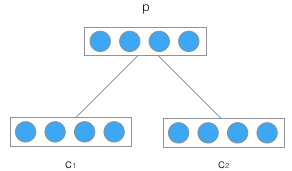
\includegraphics[width=0.5\textwidth]{Recu5.png}
	\caption{神经元两两相连}
	\label{fig:Recu5}
\end{figure}

\({c}_1\)和\({c}_2\)分别是表示两个子节点的向量,\({p}\)是表示父节点的向量。子节点和父节点组成一个全连接神经网络,也就是子节点的每个神经元都和父节点的每个神经元两两相连。我们用矩阵\(W\)表示这些连接上的权重,它的维度将是\(d\times 2d\),其中,\(d\)表示每个节点的维度。父节点的计算公式可以写成:

\begin{equation}
	\label{eq:Recu1}
	{p} = tanh(W\begin{bmatrix}{c}_1\\{c}_2\end{bmatrix}+{b})
\end{equation}


在上式中,tanh是激活函数(当然也可以用其它的激活函数),\({b}\)是偏置项,它也是一个维度为\(d\)的向量。如果读过前面的文章,相信大家已经非常熟悉这些计算了,在此不做过多的解释了。

然后,我们把产生的父节点的向量和其他子节点的向量再次作为网络的输入,再次产生它们的父节点。如此递归下去,直至整棵树处理完毕。最终,我们将得到根节点的向量,我们可以认为它是对整棵树的表示,这样我们就实现了把树映射为一个向量。在图\ref{fig:Recu6}中,我们使用\textbf{递归神经网络}处理一棵树,最终得到的向量\({p}_3\),就是对整棵树的表示:

\begin{figure}[!h]
	\centering
	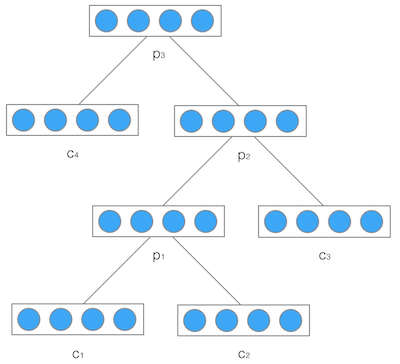
\includegraphics[width=0.5\textwidth]{Recu6.png}
	\caption{神经元树}
	\label{fig:Recu6}
\end{figure}

举个例子,我们使用\textbf{递归神将网络}将『两个外语学校的学生』映射为一个向量,如图\ref{fig:Recu7}所示:

\begin{figure}[!h]
	\centering
	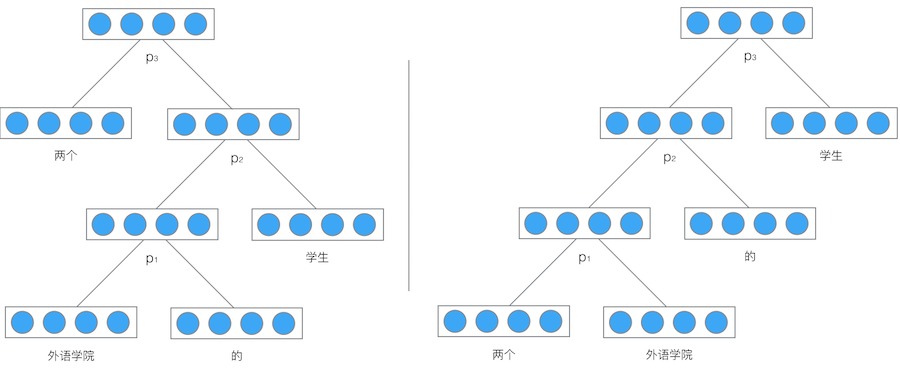
\includegraphics[width=0.8\textwidth]{Recu7.png}
	\caption{cross correlation}
	\label{神经元树映射}
\end{figure}

最后得到的向量\({p}_3\)就是对整个句子『两个外语学校的学生』的表示。由于整个结构是递归的,不仅仅是根节点,事实上每个节点都是以其为根的子树的表示。比如,在左边的这棵树中,向量\({p}_2\)是短语『外语学院的学生』的表示,而向量\({p}_1\)是短语『外语学院的』的表示。

公式\ref{eq:Recu1}就是\textbf{递归神经网络}的前向计算算法。它和全连接神经网络的计算没有什么区别,只是在输入的过程中需要根据输入的树结构依次输入每个子节点。

需要特别注意的是,\textbf{递归神经网络}的权重\(W\)和偏置项\({b}\)在所有的节点都是\textbf{共享}的。

\section{递归神经网络的训练}\label{Recu:3}

\textbf{递归神经网络}的训练算法和\textbf{循环神经网络}类似,两者不同之处在于,前者需要将残差\(\delta\)从根节点反向传播到各个子节点,而后者是将残差\(\delta\)从当前时刻\(t_k\)反向传播到初始时刻\(t_1\)。

下面,我们介绍适用于\textbf{递归神经网络}的训练算法,也就是\textbf{BPTS}算法。

\subsection{误差项的传递}\label{Recu:4}

首先,我们先推导将误差从父节点传递到子节点的公式,如图\ref{fig:Recu8}:

\begin{figure}[!h]
	\centering
	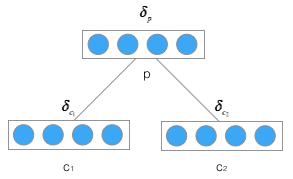
\includegraphics[width=0.5\textwidth]{Recu8.png}
	\caption{神经元树}
	\label{fig:Recu8}
\end{figure}

定义\(\delta_p\)为误差函数E相对于父节点\(p\)的加权输入\({net}_p\)的导数,即:
\[
	\delta_p\overset{def}{=}\frac{\partial{E}}{\partial{{net}_p}}
\]

设\({net}_p\)是父节点的\textbf{加权输入},则

\[{net}_p=W\begin{bmatrix}{c}_1\\{c}_2\end{bmatrix}+{b}\]

在上述式子里,\({net}_p\)、\({c}_1\)、\({c}_2\)都是向量,而\(W\)是矩阵。为了看清楚它们的关系,我们将其展开:
\begin{align*}
	\begin{bmatrix}
		net_{p_1} \\
		net_{p_2} \\
		...       \\
		net_{p_n}
	\end{bmatrix} & =
	\begin{bmatrix}
		w_{p_1c_{11}} & w_{p_1c_{12}} & ... & w_{p_1c_{1n}} & w_{p_1c_{21}} & w_{p_1c_{22}} & ... & w_{p_1c_{2n}} \\
		w_{p_2c_{11}} & w_{p_2c_{12}} & ... & w_{p_2c_{1n}} & w_{p_2c_{21}} & w_{p_2c_{22}} & ... & w_{p_2c_{2n}} \\
		...                                                                                                       \\
		w_{p_nc_{11}} & w_{p_nc_{12}} & ... & w_{p_nc_{1n}} & w_{p_nc_{21}} & w_{p_nc_{22}} & ... & w_{p_nc_{2n}} \\
	\end{bmatrix}
	\begin{bmatrix}
		c_{11} \\
		c_{12} \\
		...    \\
		c_{1n} \\
		c_{21} \\
		c_{22} \\
		...    \\
		c_{2n}
	\end{bmatrix}+\begin{bmatrix}\\
		b_1 \\
		b_2 \\
		... \\
		b_n \\
	\end{bmatrix}
\end{align*}

在上面的公式中,\(p_i\)表示父节点p的第i个分量;\(c_{1i}\)表示\(c_1\)子节点的第i个分量;\(c_{2i}\)表示\(c_2\)子节点的第i个分量;\(w_{p_ic_{jk}}\)表示子节点\(c_j\)的第k个分量到父节点p的第i个分量的的权重。根据上面展开后的矩阵乘法形式,我们不难看出,对于子节点\(c_{jk}\)来说,它会影响父节点所有的分量。因此,我们求误差函数E对\(c_{jk}\)的导数时,必须用到全导数公式,也就是:
\begin{align*}
	\frac{\partial{E}}{\partial{c_{jk}}}=\sum_i{\frac{\partial{E}}{\partial{net_{p_i}}}}\frac{\partial{net_{p_i}}}{\partial{c_{jk}}}=\sum_i{\delta_{p_i}}w_{p_ic_{jk}}
\end{align*}

有了上式,我们就可以把它表示为矩阵形式,从而得到一个向量化表达:
\begin{align*}
	\frac{\partial{E}}{\partial{{c}_j}} & =U_j\delta_p
\end{align*}

其中,矩阵\(U_j\)是从矩阵W中提取部分元素组成的矩阵。其单元为:
\[
	u_{j_{ik}}=w_{p_kc_{ji}}
\]

上式看上去可能会让人晕菜,从图\ref{fig:Recu9},我们可以直观的看到\(U_j\)到底是啥。首先我们把W矩阵拆分为两个矩阵\(W_1\)和\(W_2\)。

\begin{figure}[!h]
	\centering
	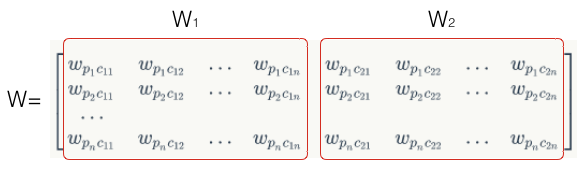
\includegraphics[width=0.9\textwidth]{Recu9.png}
	\caption{cross correlation}
	\label{fig:Recu9}
\end{figure}

显然,子矩阵\(W_1\)和\(W_2\)分别对应子节点\({c}_1\)和\({c}_2\)的到父节点\({p}\)权重。则矩阵\(U_j\)为:
\[
	U_j=W_j^T
\]

也就是说,将误差项反向传递到相应子节点\({c}_j\)的矩阵\(U_j\)就是其对应权重矩阵\(W_j\)的转置。

现在,我们设\({net}_{c_j}\)是子节点\({c}_j\)的加权输入,\(f\)是子节点c的激活函数,则:
\begin{align*}
	{c}_j=f({net}_{c_j})
\end{align*}

这样,我们得到:
\begin{align*}
	\delta_{c_j}=\frac{\partial{E}}{\partial{{net}_{c_j}}}=\frac{\partial{E}}{\partial{{c}_j}}\frac{\partial{{c}_j}}{\partial{{net}_{c_j}}}=W_j^T\delta_p\circ f'({net}_{c_j})
\end{align*}

如果我们将不同子节点\({c}_j\)对应的误差项\(\delta_{c_j}\)连接成一个向量\(\delta_c=\begin{bmatrix}\delta_{c_1}\\\delta_{c_2}\end{bmatrix}\)。那么,上式可以写成:
\begin{equation}
	\label{eq:Recu2}
	\delta_c=W^T\delta_p\circ f'({net}_c)
\end{equation}
公式\ref{eq:Recu2}就是将误差项从父节点传递到其子节点的公式。注意,上式中的\({net}_c\)也是将两个子节点的加权输入\({net}_{c_1}\)和\({net}_{c_2}\)连在一起的向量。

有了传递一层的公式,我们就不难写出逐层传递的公式。

\begin{figure}[!h]
	\centering
	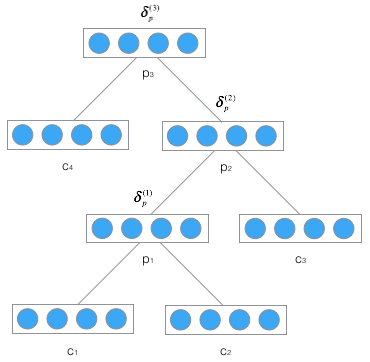
\includegraphics[width=0.6\textwidth]{Recu10.png}
	\caption{神经元树}
	\label{fig:Recu10}
\end{figure}

图\ref{fig:Recu10}是在树型结构中反向传递误差项的全景图,反复应用公式\ref{eq:Recu2},在已知\(\delta_p^{(3)}\)的情况下,我们不难算出\(\delta_p^{(1)}\)为:
\begin{align*}
	\delta^{(2)}   & =W^T\delta_p^{(3)}\circ f'({net}^{(2)}) \\
	\delta_p^{(2)} & =[\delta^{(2)}]_p                       \\
	\delta^{(1)}   & =W^T\delta_p^{(2)}\circ f'({net}^{(1)}) \\
	\delta_p^{(1)} & =[\delta^{(1)}]_p
\end{align*}

在上面的公式中,\(\delta^{(2)}=\begin{bmatrix}\delta_c^{(2)}\\\delta_p^{(2)}\end{bmatrix}\),\([\delta^{(2)}]_p\)表示取向量\(\delta^{(2)}\)属于节点p的部分。

\subsection{权重梯度的计算}\label{Recu:5}

根据加权输入的计算公式:
\[
	{net}_p^{(l)}=W{c}^{(l)}+{b}
\]

其中,\({net}_p^{(l)}\)表示第l层的父节点的加权输入,\({c}^{(l)}\)表示第l层的子节点。\(W\)是权重矩阵,\({b}\)是偏置项。将其展开可得:
\[
	{net}_{p_j}^l=\sum_i{w_{ji}c_i^l}+b_j
\]

那么,我们可以求得误差函数在第l层对权重的梯度为:
\begin{align*}
	\frac{\partial{E}}{\partial{w_{ji}^{(l)}}}=\frac{\partial{E}}{\partial{{net}_{p_j}^{(l)}}}\frac{\partial{{net}_{p_j}^{(l)}}}{\partial{w_{ji}^{(l)}}}=\delta_{p_j}^{(l)}c_i^{(l)}
\end{align*}

上式是针对一个权重项\(w_{ji}\)的公式,现在需要把它扩展为对所有的权重项的公式。我们可以把上式写成矩阵的形式(在下面的公式中,m=2n):
\begin{equation}
	\label{eq:Recu3}
	\frac{\partial{E}}{\partial{W^{(l)}}}=
	\begin{bmatrix}
		\frac{\partial{E}}{\partial{w_{11}^{(l)}}} &
		\frac{\partial{E}}{\partial{w_{12}^{(l)}}} &
		...                                        &
		\frac{\partial{E}}{\partial{w_{1m}^{(l)}}}   \\
		\frac{\partial{E}}{\partial{w_{21}^{(l)}}} &
		\frac{\partial{E}}{\partial{w_{22}^{(l)}}} &
		...                                        &
		\frac{\partial{E}}{\partial{w_{2m}^{(l)}}}   \\
		...                                          \\
		\frac{\partial{E}}{\partial{w_{n1}^{(l)}}} &
		\frac{\partial{E}}{\partial{w_{n2}^{(l)}}} &
		...                                        &
		\frac{\partial{E}}{\partial{w_{nm}^{(l)}}}   \\
	\end{bmatrix}=
	\begin{bmatrix}
		\delta_{p_1}^{(l)}c_1^l & \delta_{p_1}^{(l)}c_2^l  & ... & \delta_{p_1}^lc_m^{(l)} \\
		\delta_{p_2}^{(l)}c_1^l & \delta_{p_2}^{(l)}c_2^l  & ... & \delta_{p_2}^lc_m^{(l)} \\
		...                                                                                \\
		\delta_{p_n}^{(l)}c_1^l & \delta_{p_n}^{(l)}lc_2^l & ... & \delta_{p_n}^lc_m^{(l)} \\
	\end{bmatrix}=\delta^{{(l)}}({c}^{(l)})^T
\end{equation}

公式\ref{eq:Recu3}就是第l层权重项的梯度计算公式。我们知道,由于权重\(W\)是在所有层共享的,所以和\textbf{循环神经网络}一样,\textbf{递归神经网络}的最终的\textbf{权重梯度是各个层权重梯度之和}。即:
\begin{equation}
	\label{eq:Recu4}
	\frac{\partial{E}}{\partial{W}}=\sum_l\frac{\partial{E}}{\partial{W^{(l)}}}
\end{equation}

因为\textbf{循环神经网络}的证明过程已经在第\ref{chap:Cnn}章卷积神经网络一文中给出,因此,\textbf{递归神经网络}『为什么最终梯度是各层梯度之和』的证明就留给读者自行完成啦。

接下来,我们求偏置项\({b}\)的梯度计算公式。先计算误差函数对第l层偏置项\({b}^{(l)}\)的梯度:
\begin{align*}
	\frac{\partial{E}}{\partial{b_j^{(l)}}}=\frac{\partial{E}}{\partial{{net}_{p_j}^{(l)}}}\frac{\partial{{net}_{p_j}^{(l)}}}{\partial{b_j^{(l)}}}=\delta_{p_j}^{(l)}
\end{align*}

把上式扩展为矩阵的形式:
\begin{equation}
	\label{eq:Recu5}
	\frac{\partial{E}}{\partial{{b}^{(l)}}}=
	\begin{bmatrix}
		\frac{\partial{E}}{\partial{b_1^{(l)}}} \\
		\frac{\partial{E}}{\partial{b_2^{(l)}}} \\
		...                                     \\
		\frac{\partial{E}}{\partial{b_n^{(l)}}} \\
	\end{bmatrix}=
	\begin{bmatrix}
		\delta_{p_1}^{(l)} \\
		\delta_{p_2}^{(l)} \\
		...                \\
		\delta_{p_n}^{(l)} \\
	\end{bmatrix}=\delta_p^{{(l)}}
\end{equation}

公式\ref{eq:Recu5}是第l层偏置项的梯度,那么最终的偏置项梯度是各个层偏置项梯度之和,即:

\begin{equation}
	\label{eq:Recu6}
	\frac{\partial{E}}{\partial{{b}}}=\sum_l\frac{\partial{E}}{\partial{{b}^{(l)}}}
\end{equation}

\subsection{权重更新}\label{Recu:6}

如果使用梯度下降优化算法,那么权重更新公式为:
\[
	W\gets W + \eta\frac{\partial{E}}{\partial{W}}
\]

其中,\(\eta\)是学习速率常数。把公式\ref{eq:Recu4}带入到上式,即可完成权重的更新。同理,偏置项的更新公式为:
\[
	{b}\gets {b} + \eta\frac{\partial{E}}{\partial{{b}}}
\]

把公式\ref{eq:Recu6}带入到上式,即可完成偏置项的更新。

这就是\textbf{递归神经网络}的训练算法BPTS。由于我们有了前面几篇文章的基础,相信读者们理解BPTS算法也会比较容易。

\section{编程实战:递归神经网络的实现}\label{Recu:7}

\begin{note}
	完整代码请参考GitHub:\url{https://github.com/hanbt/learn_dl/blob/master/recursive.py}(python2.7)
\end{note}

现在,我们实现一个处理树型结构的\textbf{递归神经网络}。

在文件的开头,加入如下代码:
\begin{lstlisting}
#!/usr/bin/env python
# -*- coding: UTF-8 -*-
import numpy as np
from cnn import IdentityActivator
\end{lstlisting}


上述四行代码非常简单,没有什么需要解释的。IdentityActivator激活函数是在我们介绍\textbf{卷积神经网络}时写的,现在引用一下它。

我们首先定义一个树节点结构,这样,我们就可以用它保存卷积神经网络生成的整棵树:
\begin{lstlisting}
class TreeNode(object):
    def __init__(self, data, children=[], children_data=[]):
        self.parent = None
        self.children = children
        self.children_data = children_data
        self.data = data
        for child in children:
            child.parent = self
\end{lstlisting}


接下来,我们把\textbf{递归神经网络}的实现代码都放在RecursiveLayer类中,下面是这个类的构造函数:
\begin{lstlisting}
# 递归神经网络实现
class RecursiveLayer(object):
    def __init__(self, node_width, child_count, 
                 activator, learning_rate):
        '''
        递归神经网络构造函数
        node_width: 表示每个节点的向量的维度
        child_count: 每个父节点有几个子节点
        activator: 激活函数对象
        learning_rate: 梯度下降算法学习率
        '''
        self.node_width = node_width
        self.child_count = child_count
        self.activator = activator
        self.learning_rate = learning_rate
        # 权重数组W
        self.W = np.random.uniform(-1e-4, 1e-4,
            (node_width, node_width * child_count))
        # 偏置项b
        self.b = np.zeros((node_width, 1))
        # 递归神经网络生成的树的根节点
        self.root = None
\end{lstlisting}


下面是前向计算的实现:
\begin{lstlisting}
    def forward(self, *children):
        '''
        前向计算
        '''
        children_data = self.concatenate(children)
        parent_data = self.activator.forward(
            np.dot(self.W, children_data) + self.b
        )
        self.root = TreeNode(parent_data, children
                            , children_data)
\end{lstlisting}


forward函数接收一系列的树节点对象作为输入,然后,\textbf{递归神经网络}将这些树节点作为子节点,并计算它们的父节点。最后,将计算的父节点保存在self.root变量中。

上面用到的concatenate函数,是将各个子节点中的数据拼接成一个长向量,其代码如下:
\begin{lstlisting}
    def concatenate(self, tree_nodes):
        '''
        将各个树节点中的数据拼接成一个长向量
        '''
        concat = np.zeros((0,1))
        for node in tree_nodes:
            concat = np.concatenate((concat, node.data))
        return concat
\end{lstlisting}

下面是反向传播算法BPTS的实现:
\begin{lstlisting}
    def backward(self, parent_delta):
        '''
        BPTS反向传播算法
        '''
        self.calc_delta(parent_delta, self.root)
        self.W_grad, self.b_grad = self.calc_gradient(self.root)
    def calc_delta(self, parent_delta, parent):
        '''
        计算每个节点的delta
        '''
        parent.delta = parent_delta
        if parent.children:
            # 根据式2计算每个子节点的delta
            children_delta = np.dot(self.W.T, parent_delta) * (
                self.activator.backward(parent.children_data)
            )
            # slices = [(子节点编号,子节点delta起始位置,子节点delta结束位置)]
            slices = [(i, i * self.node_width, 
                        (i + 1) * self.node_width)
                        for i in range(self.child_count)]
            # 针对每个子节点,递归调用calc_delta函数
            for s in slices:
                self.calc_delta(children_delta[s[1]:s[2]], 
                                parent.children[s[0]])
    def calc_gradient(self, parent):
        '''
        计算每个节点权重的梯度,并将它们求和,得到最终的梯度
        '''
        W_grad = np.zeros((self.node_width, 
                            self.node_width * self.child_count))
        b_grad = np.zeros((self.node_width, 1))
        if not parent.children:
            return W_grad, b_grad
        parent.W_grad = np.dot(parent.delta, parent.children_data.T)
        parent.b_grad = parent.delta
        W_grad += parent.W_grad
        b_grad += parent.b_grad
        for child in parent.children:
            W, b = self.calc_gradient(child)
            W_grad += W
            b_grad += b
        return W_grad, b_grad
\end{lstlisting}


在上述算法中,calc\_delta函数和calc\_gradient函数分别计算各个节点的误差项\(\delta\)以及最终的梯度。它们都采用递归算法,先序遍历整个树,并逐一完成每个节点的计算。

下面是梯度下降算法的实现(没有weight decay),这个非常简单:
\begin{lstlisting}
    def update(self):
        '''
        使用SGD算法更新权重
        '''
        self.W -= self.learning_rate * self.W_grad
        self.b -= self.learning_rate * self.b_grad
\end{lstlisting}


以上就是\textbf{递归神经网络}的实现,总共100行左右,和上一篇文章的LSTM相比简单多了。

最后,我们用梯度检查来验证程序的正确性:
\begin{lstlisting}
    def gradient_check():
    '''
    梯度检查
    '''
    # 设计一个误差函数,取所有节点输出项之和
    error_function = lambda o: o.sum()
    rnn = RecursiveLayer(2, 2, IdentityActivator(), 1e-3)
    # 计算forward值
    x, d = data_set()
    rnn.forward(x[0], x[1])
    rnn.forward(rnn.root, x[2])
    # 求取sensitivity map
    sensitivity_array = np.ones((rnn.node_width, 1),
                                dtype=np.float64)
    # 计算梯度
    rnn.backward(sensitivity_array)
    # 检查梯度
    epsilon = 10e-4
    for i in range(rnn.W.shape[0]):
        for j in range(rnn.W.shape[1]):
            rnn.W[i,j] += epsilon
            rnn.reset_state()
            rnn.forward(x[0], x[1])
            rnn.forward(rnn.root, x[2])
            err1 = error_function(rnn.root.data)
            rnn.W[i,j] -= 2*epsilon
            rnn.reset_state()
            rnn.forward(x[0], x[1])
            rnn.forward(rnn.root, x[2])
            err2 = error_function(rnn.root.data)
            expect_grad = (err1 - err2) / (2 * epsilon)
            rnn.W[i,j] += epsilon
            print 'weights(%d,%d): expected - actural %.4e - %.4e' % (
                i, j, expect_grad, rnn.W_grad[i,j])
    return rnn
\end{lstlisting}


下面是梯度检查的结果,完全正确,OH YEAH!

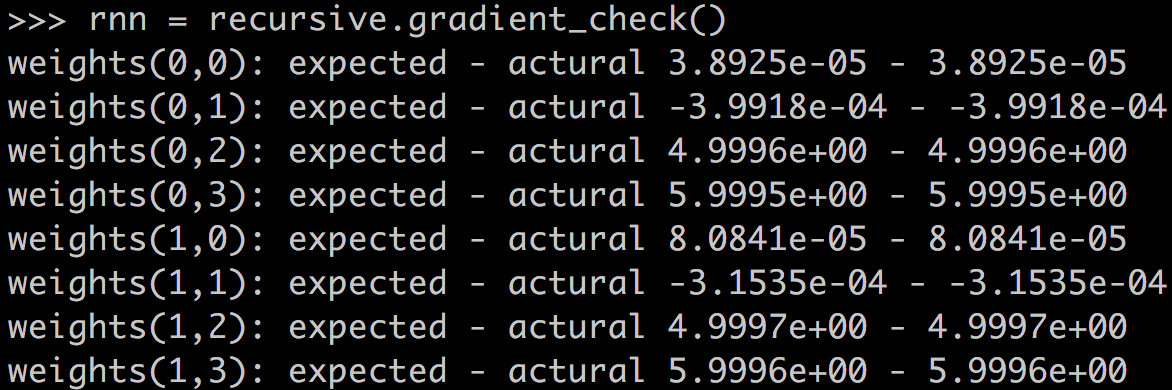
\includegraphics[width=0.8\textwidth]{Recu11.png}

\section{递归神经网络的应用}\label{Recu:8}
\subsection{自然语言和自然场景解析}\label{Recu:9}

在自然语言处理任务中,如果我们能够实现一个解析器,将自然语言解析为语法树,那么毫无疑问,这将大大提升我们对自然语言的处理能力。解析器如图\ref{fig:Recu12}所示:

\begin{figure}[!h]
	\centering
	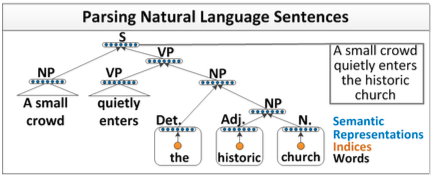
\includegraphics[width=0.65\textwidth]{Recu12.png}
	\caption{解析器}
	\label{fig:Recu12}
\end{figure}

可以看出,\textbf{递归神经网络}能够完成句子的语法分析,并产生一个语法解析树。

除了自然语言之外,自然场景也具有\textbf{可组合}的性质。因此,我们可以用类似的模型完成自然场景的解析,如图\ref{fig:Recu13}所示:

\begin{figure}[!h]
	\centering
	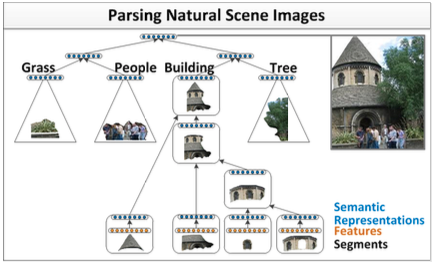
\includegraphics[width=0.6\textwidth]{Recu13.png}
	\caption{自然场景的解析}
	\label{fig:Recu13}
\end{figure}

两种不同的场景,可以用相同的\textbf{递归神经网络}模型来实现。我们以第一个场景,自然语言解析为例。

我们希望将一句话逐字输入到神经网络中,然后,神经网络返回一个解析好的树。为了做到这一点,我们需要给神经网络再加上一层,负责打分。分数越高,说明两个子节点结合更加紧密,分数越低,说明两个子节点结合更松散。如图\ref{fig:Recu14}所示:

\begin{figure}[!h]
	\centering
	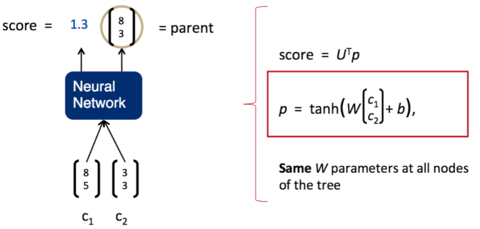
\includegraphics[width=0.7\textwidth]{Recu14.png}
	\caption{两个子节点}
	\label{fig:Recu14}
\end{figure}

一旦这个打分函数训练好了(也就是矩阵U的各项值变为合适的值),我们就可以利用贪心算法来实现句子的解析。第一步,我们先将词按照顺序两两输入神经网络,得到第一组打分:

\begin{figure}[!h]
	\centering
	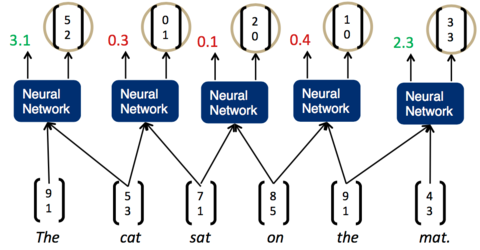
\includegraphics[width=0.7\textwidth]{Recu15.png}
	\caption{输入神经网络}
	\label{fig:Recu15}
\end{figure}

我们发现,现在分数最高的是第一组,The cat,说明它们的结合是最紧密的。这样,我们可以先将它们组合为一个节点。然后,再次两两计算相邻子节点的打分:

\begin{figure}[!h]
	\centering
	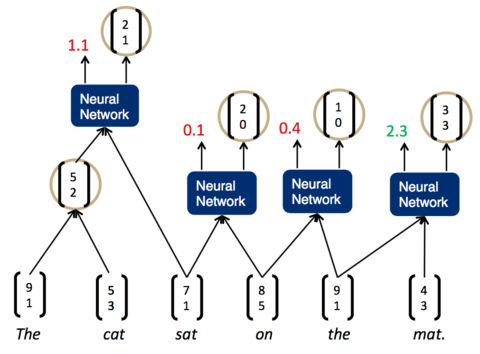
\includegraphics[width=0.8\textwidth]{Recu16.png}
	\caption{相邻子节点的打分}
	\label{fig:Recu16}
\end{figure}

现在,分数最高的是最后一组,the mat。于是,我们将它们组合为一个节点,再两两计算相邻节点的打分:

\begin{figure}[!h]
	\centering
	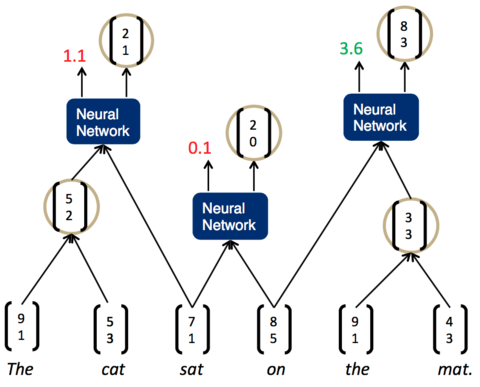
\includegraphics[width=0.8\textwidth]{Recu17.png}
	\caption{相邻子节点的打分}
	\label{fig:Recu17}
\end{figure}

这时,我们发现最高的分数是on the mat,把它们组合为一个节点,继续两两计算相邻节点的打分......最终,我们就能够得到整个解析树:

\begin{figure}[!h]
	\centering
	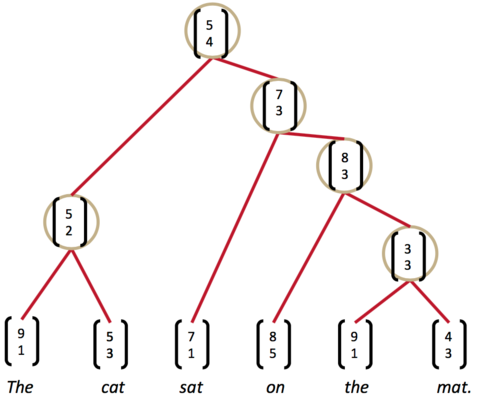
\includegraphics[width=0.7\textwidth]{Recu18.png}
	\caption{整个解析树}
	\label{fig:Recu18}
\end{figure}

现在,我们困惑这样牛逼的打分函数score是怎样训练出来的呢?我们需要定义一个目标函数。这里,我们使用Max-Margin目标函数。它的定义如下:
\[
	J(\theta)=max(0, \sum_i\underset{y\in A(x_i)}{max}(s(x_i,y)+\Delta(y,y_i))-s(x_i,y_i))
\]

在上式中,\(x_i\)、\(y_i\)分别表示第i个训练样本的输入和标签,注意这里的标签\(y_i\)是一棵解析树。\(s(x_i,y_i)\)就是打分函数s对第i个训练样本的打分。因为训练样本的标签肯定是正确的,我们希望s对它的打分越高越好,也就是\(s(x_i,y_i)\)越大越好。\(A(x_1)\)是所有可能的解析树的集合,而\(s(x_i,y)\)则是对某个可能的解析树\(y\)的打分。\(\Delta(y,y_i)\)是对错误的惩罚。也就是说,如果某个解析树\(y\)和标签\(y_i\)是一样的,那么\(\Delta(y,y_i)\)为0,如果网络的输出错的越离谱,那么惩罚项\(\Delta(y,y_i)\)的值就越高。\(max(s(x_i,y)+\Delta(y,y_i))\)表示所有树里面最高得分。在这里,惩罚项相当于Margin,也就是我们虽然希望打分函数s对正确的树打分比对错误的树打分高,但也不要高过Margin的值。我们优化\(\theta\),使目标函数取最小值,即:
\[
	\theta=\underset{\theta}{argmin}J(\theta)
\]

下面是惩罚函数\(\Delta\)的定义:
\[
	\Delta(y,y_i)=k\sum_{d\in N(y)}{1}{\{subTree(d)\notin y_i\}}
\]

上式中,N(y)是树y节点的集合;subTree(d)是以d为节点的子树。上式的含义是,如果以d为节点的子树没有出现在标签\(y_i\)中,那么函数值+1。最终,惩罚函数的值,是树y中没有出现在树\(y_i\)中的子树的个数,再乘上一个系数k。其实也就是关于两棵树差异的一个度量。

\(s(x,y)\)是对一个样本最终的打分,它是对树y每个节点打分的总和。
\[
	s(x,y)=\sum_{n\in nodes(y)}s_n
\]

具体细节,读者可以查阅『参考资料3』的论文。

\section{小结}

我们在系列文章中已经介绍的\textbf{全连接神经网络}、\textbf{卷积神经网络}、\textbf{循环神经网络}和\textbf{递归神经网络},在训练时都使用了\textbf{监督学习(Supervised
	Learning)}作为训练方法。在\textbf{监督学习}中,每个训练样本既包括输入特征\({x}\),也包括标记\({y}\),即样本\(d^{(i)}=\{{x}^{(i)},{y}^{(i)}\}\)。然而,很多情况下,我们无法获得形如\(\{{x}^{(i)},{y}^{(i)}\}\)的样本,这时,我们就不能采用\textbf{监督学习}的方法。在接下来的几篇文章中,我们重点介绍另外一种学习方法:\textbf{增强学习 Reinforcement Learning)}。在了解\textbf{增强学习}的主要算法之后,我们还将介绍著名的围棋软件\textbf{AlphaGo},它是一个把\textbf{监督学习}和\textbf{增强学习}进行完美结合的案例。

